%auto-ignore
\section{Appendix.}

\subsection{Base Model Configurations}
\label{sec:base_configs}
Our base model configuration for our largest model of size 3B parameters is given in \tabb{basemodel}.

%auto-ignore
\begin{table}[ht!]
\tablestyle{6pt}{1.02}
\scriptsize
\begin{tabular}{y{107}|y{150}}
Configuration & Value \\
\shline

Number of Transformer layers & 48 \\
Transformer Hidden Dimension & 2048 \\
Transformer MLP Dimension & 8192 \\ 
Optimizer & AdaFactor \citep{shazeer2018adafactor} \\
Base learning rate & 1e-4 \\
Weight decay  & 0.045 \\
Optimizer momentum & $\beta_1{=}0.9, \beta_2{=}0.96$ \\
Batch size & 512 \\
Learning rate schedule & cosine decay \citep{Loshchilov2017SGDRSG} \\
Warmup steps & 5000 \\
Training steps & 1.5M 

\end{tabular}
\vspace{-.5em}
\caption{Configuration and training hyperparameters for base model.}
\label{tab:basemodel} \vspace{-.5em}
\end{table}

\subsection{VQGAN Configurations}
\label{sec:vqgan_configs}

%auto-ignore
\begin{table}[ht!]
\tablestyle{6pt}{1.02}
\scriptsize
\begin{tabular}{y{107}|y{150}}
Configuration & Value \\
\shline

Perceptual loss weight & 0.05 \\
Adversarial loss weight & 0.1 \\
Codebook size & 8192 \\
Optimizer & Adam \citep{KingmaB14} \\
Discriminator learning rate & 1e-4 \\
Generator learning rate & 1e-4 \\
Weight decay  & 1e-4 \\
Optimizer momentum & $\beta_1{=}0.9, \beta_2{=}0.99$ \\
Batch size & 256 \\
Learning rate schedule & cosine decay \citep{Loshchilov2017SGDRSG} \\
Warmup steps \citep{Goyal2017AccurateLM} & 10000 \\
Training steps & 1M

\end{tabular}
\vspace{-.5em}
\caption{Configuration and training hyperparameters for VQGAN.}
\label{tab:vqgan} \vspace{-.5em}
\end{table}

\textbf{VQGAN Architecture}: Our VQGAN architecture is similar to the previous work \citep{esser2021taming}. It consists of several residual blocks, downsample(encoder) and upsample (decoder) blocks. The main difference is that we remove the non-local block to make the encoder and decoder fully convolutional to support different image sizes. In the base VQGAN model, we apply 2 residual blocks in each resolution and the base channel dimension is 128. For the finetuned decoder, we apply 4 residual blocks in each resolution and we also make the base channel dimension to be 256. 


\begin{figure*}[ht!]
\centering
\begin{tabularx}{0.92\textwidth}{c c c}
%\begin{tabularx}{}
%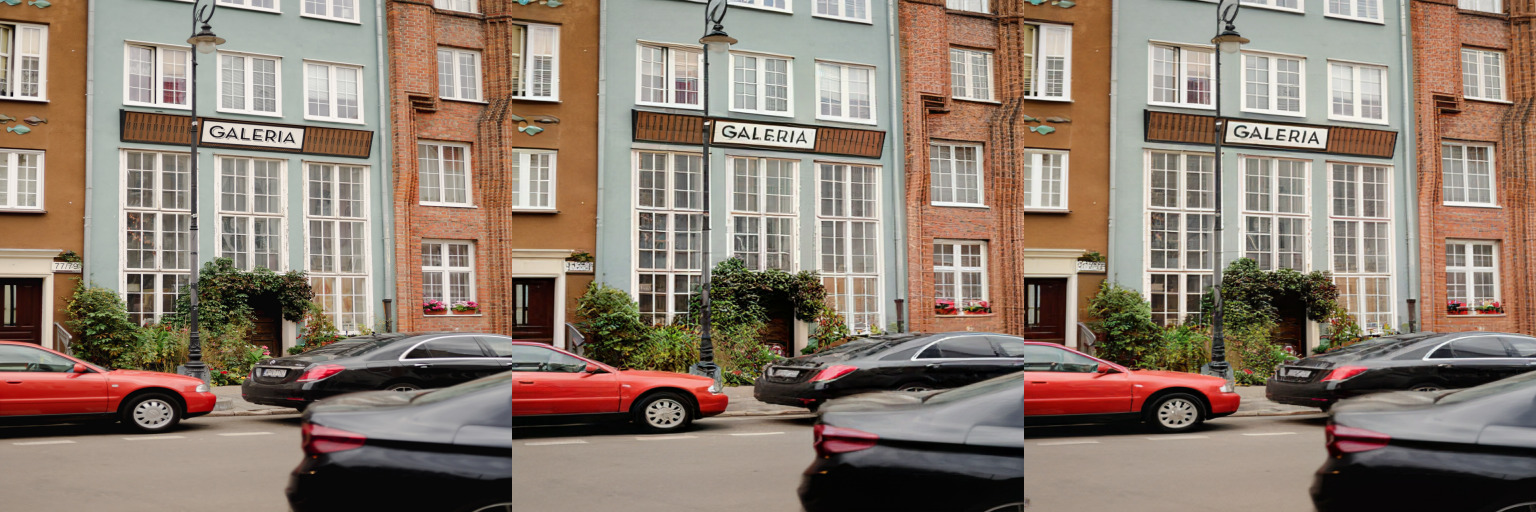
\includegraphics[width=0.90\textwidth]{figs/fine_tune_decoder/free6_grid}
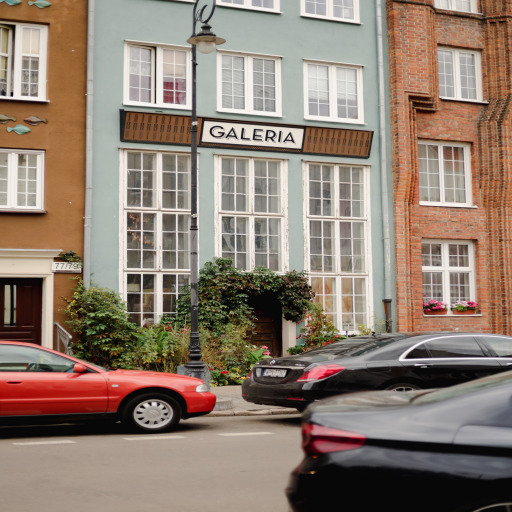
\includegraphics[width=0.30\textwidth]{figs/fine_tune_decoder/free6_ori} &
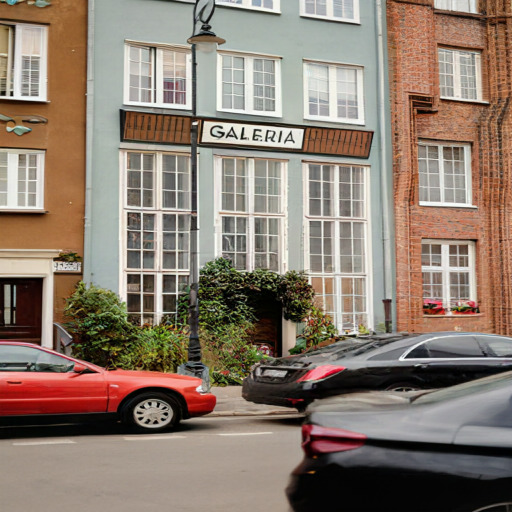
\includegraphics[width=0.30\textwidth]{figs/fine_tune_decoder/free6_reconstruced} &
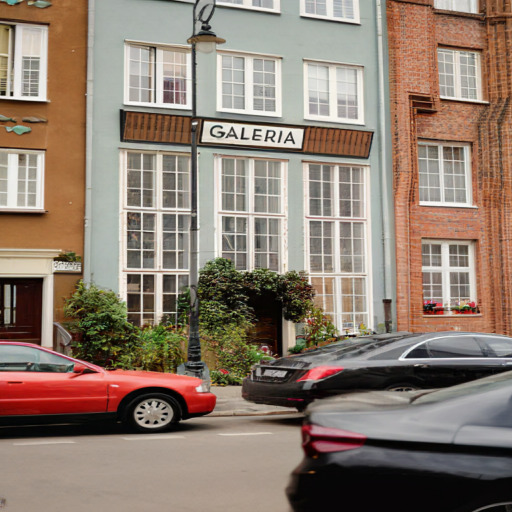
\includegraphics[width=0.30\textwidth]{figs/fine_tune_decoder/free6_ft_reconstruced}

\\
Input Image &
VQGAN Reconstruction &
Finetuned Decoder 

\end{tabularx}
\caption{\small Visual example of the improvement from the fine-tuned decoder (\cref{sec:dec_finetune}). Please zoom in by at least 200\% to see the difference between the VQGAN reconstruction and the reconstruction with a finetuned decoder. We can see especially that fine details such as the house number (bottom left), the storefront sign (middle) and the bars on the windows (right) are better preserved in the finetuned decoder.}
\label{fig:finetune_decoder}
\end{figure*}



\subsection{Super Resolution Configurations}
\label{sec:superres_configs}

%auto-ignore
\begin{table}[ht!]
\tablestyle{6pt}{1.02}
\scriptsize
\begin{tabular}{y{107}|y{150}}
Configuration & Value \\
\shline
LowRes Encoder Transformer Layers & 16 \\
Number of Transformer layers & 32 \\
Transformer Hidden Dimension & 1024 \\
Transformer MLP Dimension & 4096 \\ 
Optimizer & AdaFactor \citep{shazeer2018adafactor} \\
Base learning rate & 1e-4 \\
Weight decay  & 0.045 \\
Optimizer momentum & $\beta_1{=}0.9, \beta_2{=}0.96$ \\
Batch size & 512 \\
Learning rate schedule & cosine decay \citep{Loshchilov2017SGDRSG} \\
Warmup steps & 5000 \\
Training steps & 1M

\end{tabular}
\vspace{-.5em}
\caption{Configuration and training hyperparameters for the Super-Resolution Model.}
\label{tab:superres} \vspace{-.5em}
\end{table}
